
\begin{frame}
  \frametitle{Prediction Using Processed Gamma Spectra}
  \begin{adjustwidth}{-10pt}{-10pt}
  \begin{minipage}{0.5\textwidth}
    \begin{block}{Reactor Parameter Prediction Using \textbf{Nuclide Masses}}
      \begin{figure}
        \centering
        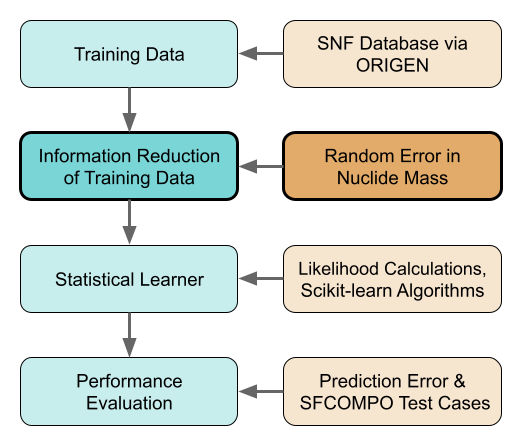
\includegraphics[width=\textwidth]{./figures/methodology1_pres.png}
      \end{figure}
    \end{block}
  \end{minipage}%
  \hfill
  \begin{minipage}{0.5\textwidth}
    \begin{block}{Reactor Parameter Prediction Using \textbf{Processed Gamma Spectra}}
      \begin{figure}
        \centering
        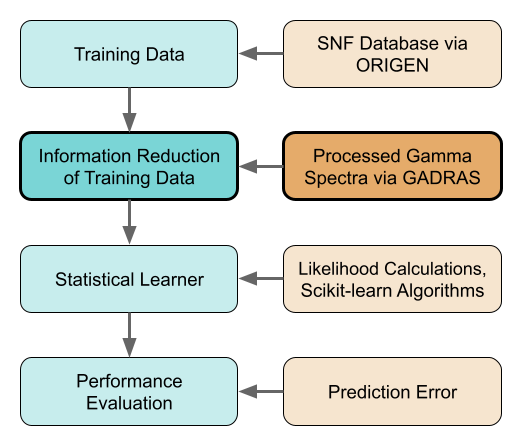
\includegraphics[width=\textwidth]{./figures/methodology2_pres.png}
      \end{figure}
    \end{block}
  \end{minipage}
  \end{adjustwidth}
\end{frame}

\begin{frame}
  \frametitle{Information Reduction: Processed Gamma Spectra}
  \begin{enumerate}
    \item Computational gamma detection \cite{gadras} 
    \item Process spectra: choose energy windows / window size
    \item Apply statistical counting error ($\sqrt{n}$) (using methods on previous slide)
  \end{enumerate}
  \begin{figure}
    \centering
    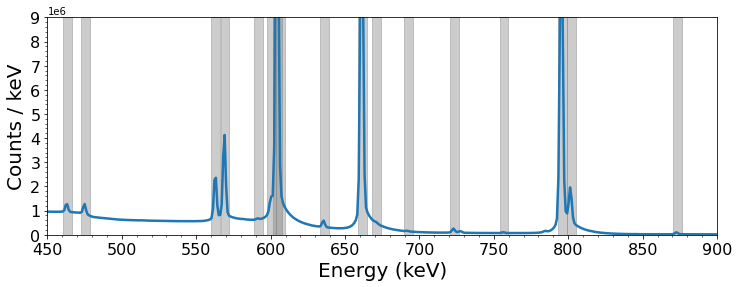
\includegraphics[width=\textwidth]{./figures/energy_window_example.png}
  \end{figure}
\end{frame}

\begin{frame}
  \frametitle{Gamma Spectra Processing}
  \begin{table}
    \small
    \centering
    \begin{tabular}{@{}lcm{0.5in}m{0.5in}m{0.5in}@{}}
      \toprule
      \multirow{2}{*}{\textbf{Detector}} &
      \multirow{2}{*}{\textbf{\begin{tabular}[c]{@{}l@{}}Energy Window\\ Size {[keV]}\end{tabular}}} &
      \multicolumn{3}{c}{\textbf{\# of Energy Windows}} \\ \cmidrule(l){3-5}
                       &    & Auto & Short & Long \\
      \toprule
      In-Lab HPGe      & 2  & 206  & 42    & 151  \\
      Portable HPGe    & 3  & 120  & 42    & 151  \\
      CZT              & 8  & 30   & 42    & 151  \\
      $\text{SrI}_2$   & 10 & 17   & 42    & 151  \\
      $\text{LaBr}_3$  & 12 & 19   & 42    & 151  \\
      NaI              & 12 & 9    & 42    & 151  \\ 
      \bottomrule
    \end{tabular}
  \end{table}
  \begin{table}
    \centering
    \renewcommand{\arraystretch}{1.3}
    \begin{tabular}{@{}|l|l|l|@{}}
      \hline
      \allbold{${}^{241}\text{Am}$} & \allbold{${}^{243}\text{Am}$} & ${}^{243}\text{Cm}$           \\ \hline
      ${}^{244}\text{Cm}$           & ${}^{245}\text{Cm}$           & \allbold{${}^{134}\text{Cs}$} \\ \hline
      \allbold{${}^{137}\text{Cs}$} & ${}^{152}\text{Eu}$           & \allbold{${}^{154}\text{Eu}$} \\ \hline
      \allbold{${}^{85}\text{Kr}$}  & ${}^{238}\text{Pu}$           & \allbold{${}^{125}\text{Sb}$} \\ \hline
    \end{tabular}
  \end{table}
\end{frame}

\begin{frame}
  \frametitle{Reactor Type Classification}
  \begin{adjustwidth}{-15pt}{-10pt}
  \begin{figure}
    \centering
    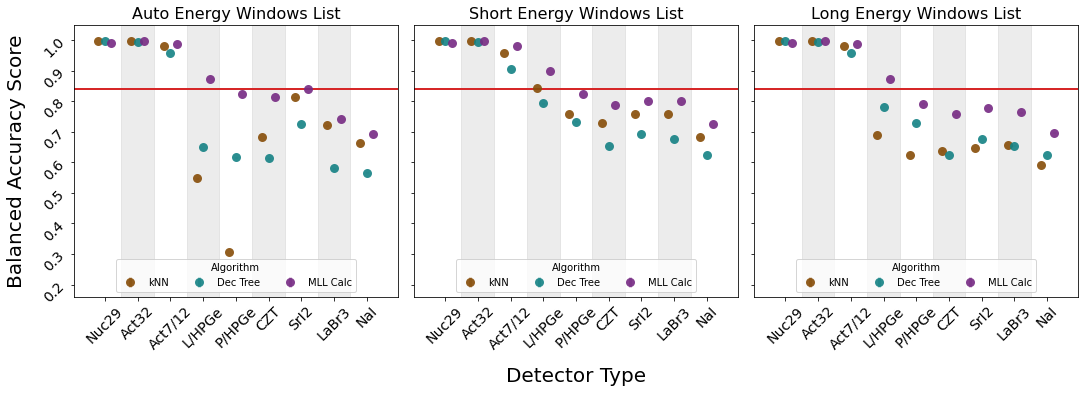
\includegraphics[width=1.1\textwidth]{./figures/detector_preds_wrt_enlist_BalAcc_rxtr.png}
    \scriptsize (99.9\% confidence interval error bars)
  \end{figure}
  \vspace{12pt} \centering Red baseline: 0.84 balanced accuracy score
  \end{adjustwidth}
\end{frame}

\begin{frame}
  \frametitle{Reactor Type Classification}
  \begin{minipage}{0.5\textwidth}
    \begin{figure}
      \centering
      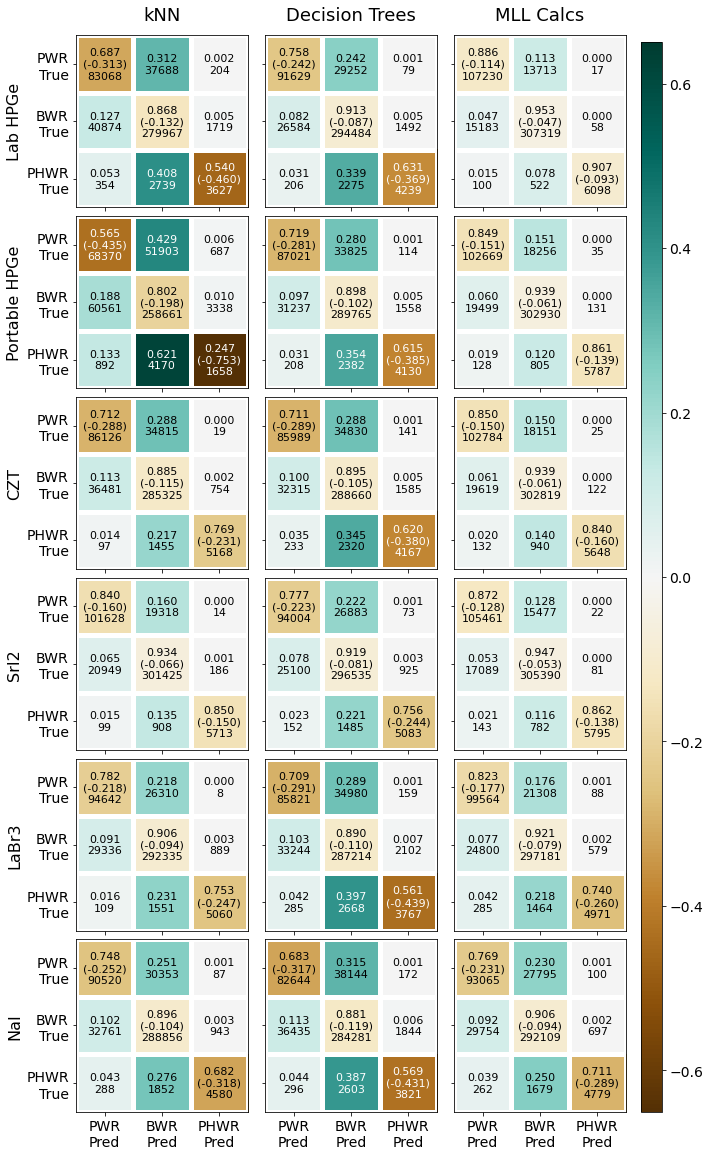
\includegraphics[height=0.88\textheight]{./figures/confusion_matrix_6dets_auto.png}
    \end{figure}
  \end{minipage}%
  \begin{minipage}{0.5\textwidth}
    \begin{figure}
      \centering
      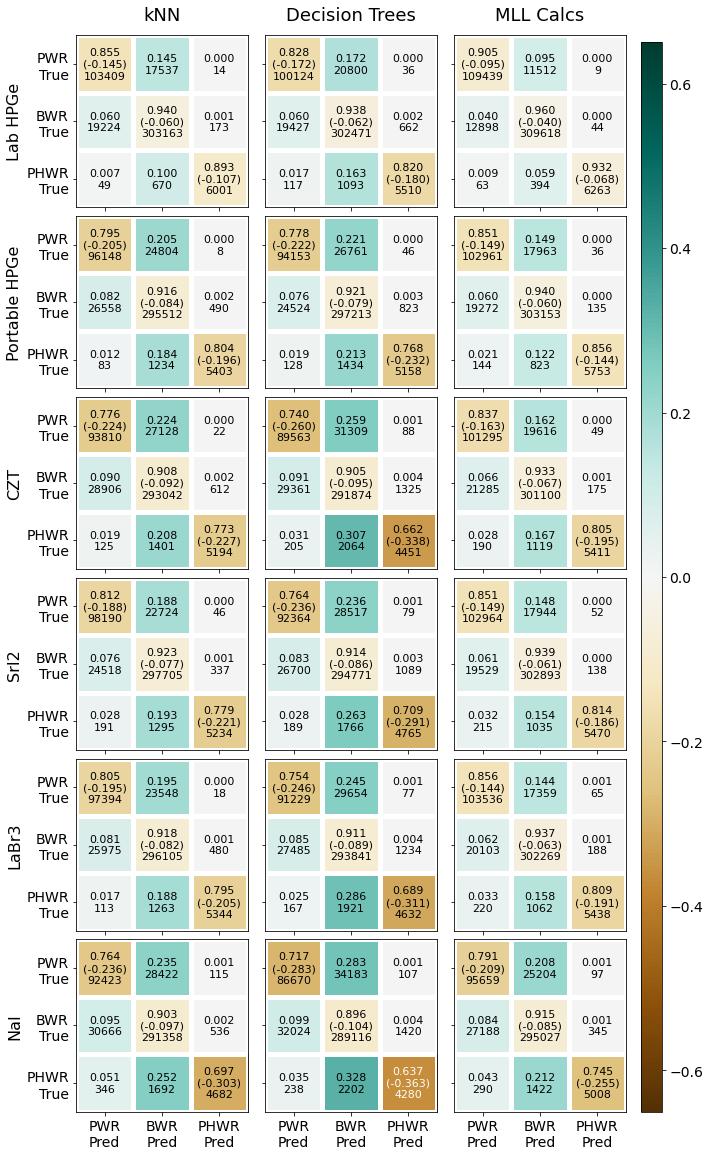
\includegraphics[height=0.88\textheight]{./figures/confusion_matrix_6dets_short.png}
    \end{figure}
  \end{minipage}
\end{frame}

\begin{frame}
  \frametitle{Burnup Regression}
  \begin{adjustwidth}{-15pt}{-10pt}
  \begin{figure}
    \centering
    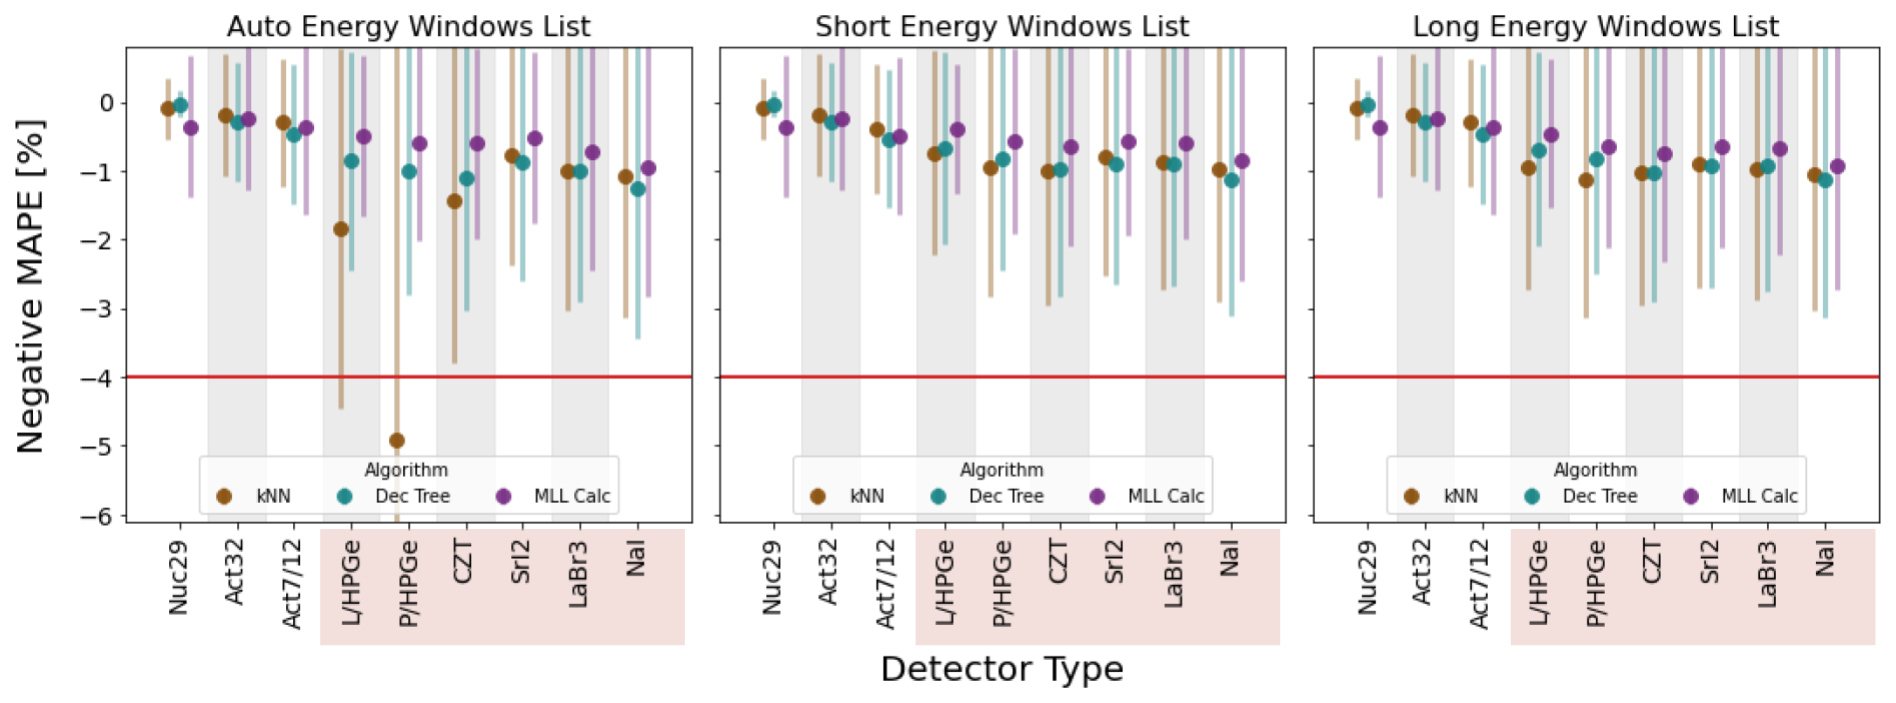
\includegraphics[width=1.1\textwidth]{./figures/detector_preds_wrt_enlist_MAPE_burn.png}
    \scriptsize (1-sigma error bars)
  \end{figure}
  \vspace{12pt} \centering Red baseline: -4\% 
  \end{adjustwidth}
\end{frame}

\begin{frame}
  \frametitle{${}^{235}\text{U}$ Enrichment Regression}
  \begin{adjustwidth}{-15pt}{-10pt}
  \begin{figure}
    \centering
    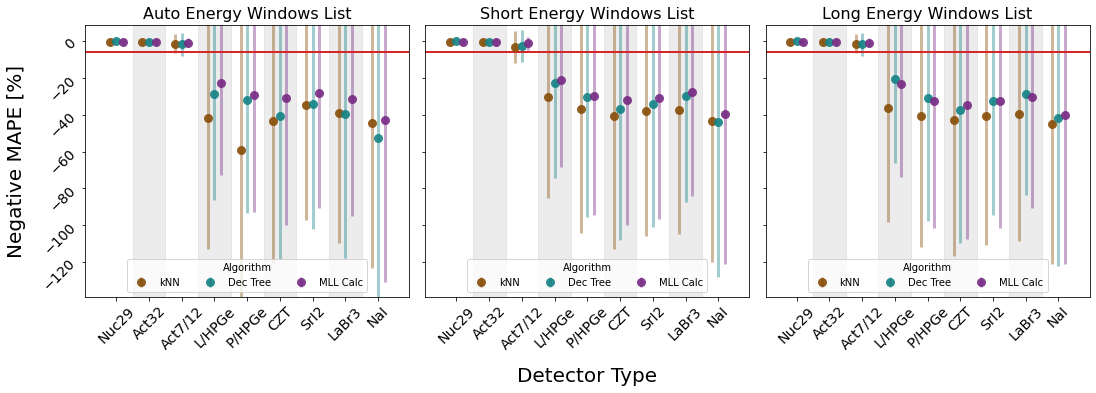
\includegraphics[width=1.1\textwidth]{./figures/detector_preds_wrt_enlist_MAPE_enri.png}
    \scriptsize (1-sigma error bars)
  \end{figure}
  \vspace{12pt} \centering Red baseline: -6\% 
  \end{adjustwidth}
\end{frame}

\begin{frame}
  \frametitle{Time Since Irradiation Regression}
  \begin{adjustwidth}{-15pt}{-10pt}
  \begin{figure}
    \centering
    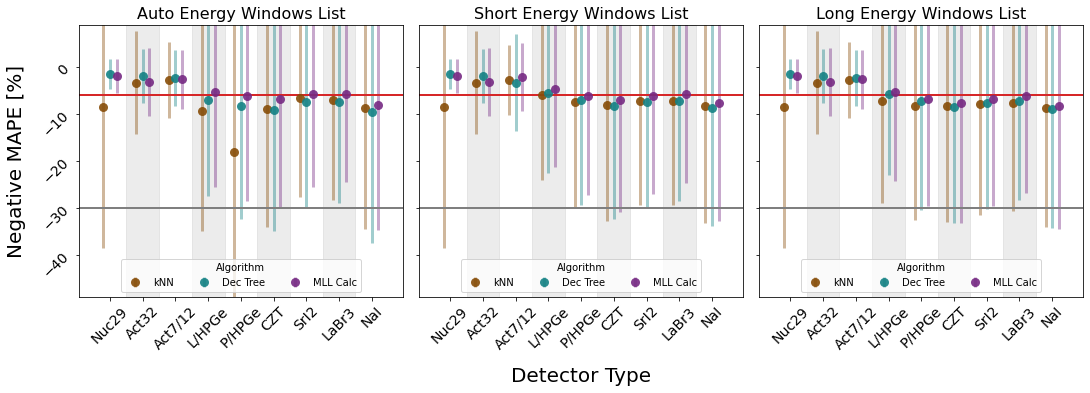
\includegraphics[width=1.1\textwidth]{./figures/detector_preds_wrt_enlist_MAPE_cool.png}
    \scriptsize (1-sigma error bars)
  \end{figure}
  \vspace{12pt} \centering Red baseline: -6\% (Grey line is -30\%) 
  \end{adjustwidth}
\end{frame}

\begin{frame}
  \frametitle{Time Since Irradiation Regression}
  \begin{adjustwidth}{-15pt}{-10pt}
  \begin{figure}
    \centering
    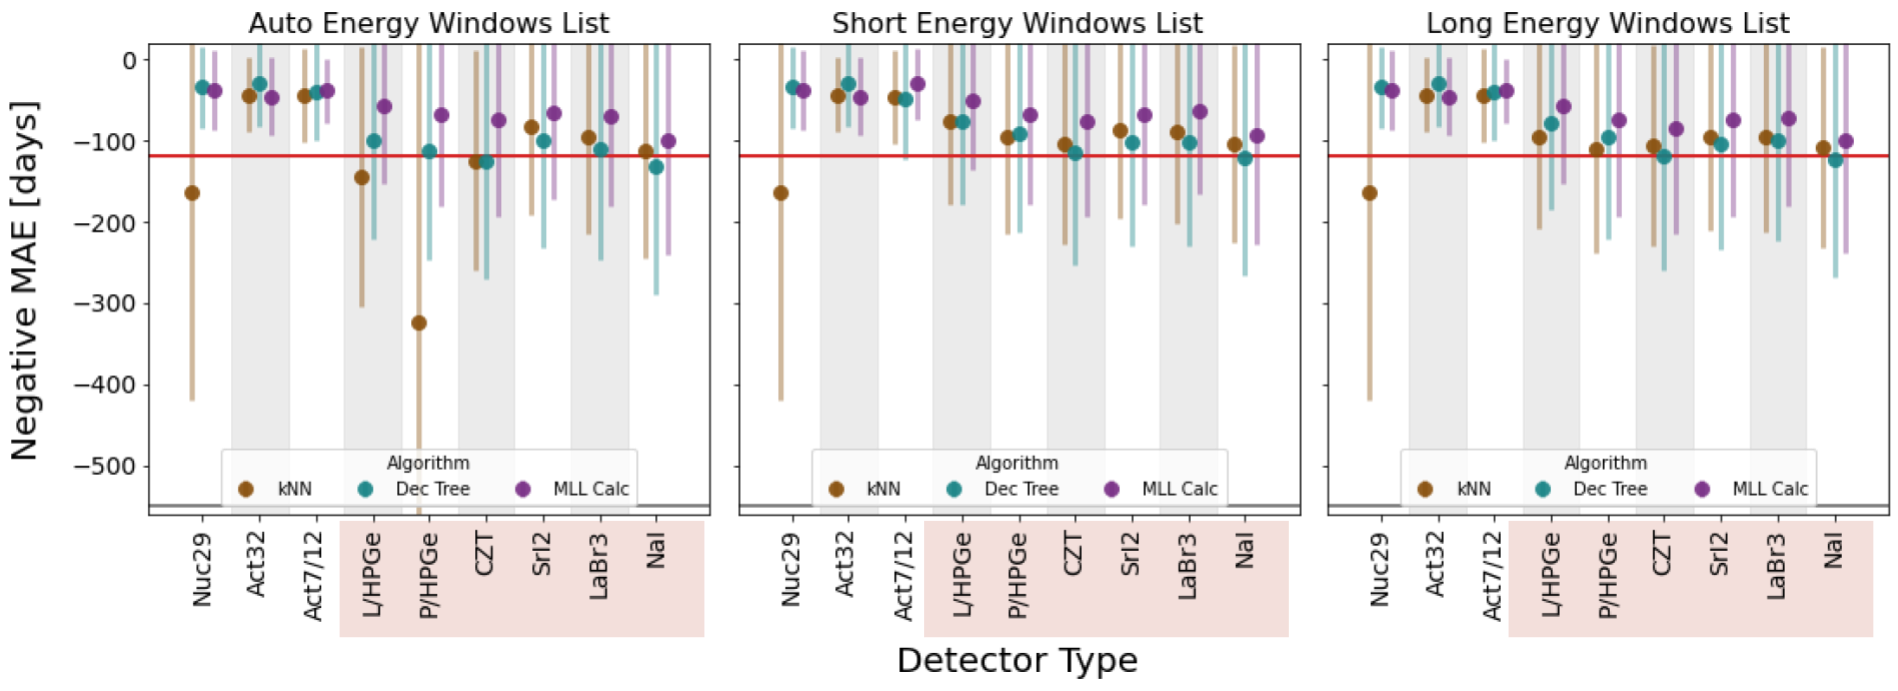
\includegraphics[width=1.1\textwidth]{./figures/detector_preds_wrt_enlist_MAE_cool.png}
    \scriptsize (1-sigma error bars)
  \end{figure}
  \vspace{12pt} \centering Red baseline: -120 $days$ (Grey line is -550 $days$)
  \end{adjustwidth}
\end{frame}

\begin{frame}
  \frametitle{Experiment Summary}
  \begin{itemize}
    \item Reactor type classification only exceeds threshold for four detector
    cases
    \item Burnup regression well exceeds the standard
    \item ${}^{235}\text{U}$ enrichment regression performs well below the
    standard
    \item Time since irradiation regression performs on or near the baseline
    \item Results are for the most part independent of gamma spectra processing 
    approach
  \end{itemize}
\end{frame}

